\begin{frame}{CSS: Warum „Spread Spectrum“?}
  Ein Chirp belegt im Spektrum eine Bandbreite $BW = \Delta f_c = f_c^{max} - f_c^{min}$.
  \begin{columns}[onlytextwidth]
    \begin{column}{0.5\textwidth}
    \begin{figure}
    Zeitbereich: Signal $g$\\
    Chirp (\SI{0.1}{\second}, \num{500} -- \SI{4000}{\hertz}, $f_s = \SI{10}{\kilo\hertz}$)
    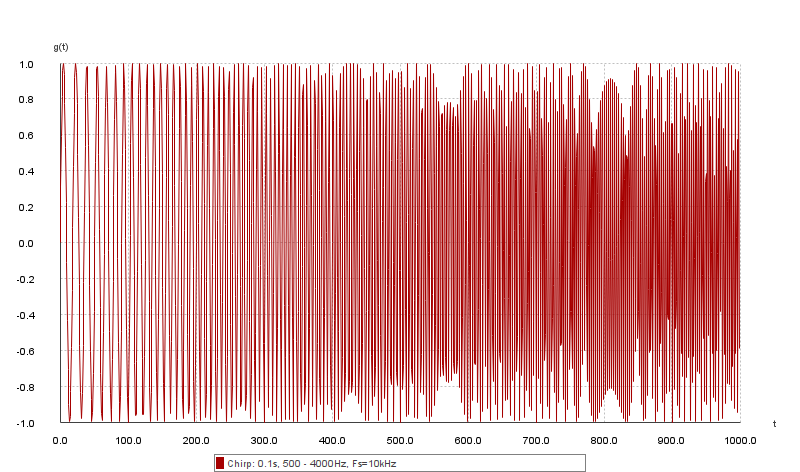
\includegraphics[width=\textwidth]{material/Aufgabe 6.1.1.png}
    \caption{Zeitverlauf des Signals $g$.}
    \end{figure}
    \end{column}
    \begin{column}{0.5\textwidth}
    \begin{figure}
    Frequenzbereich: $\mathscr{F}(g)$\\
    Chirp (\SI{1}{\second}, \num{500} -- \SI{4000}{\hertz}, $f_s = \SI{10}{\kilo\hertz}$)
    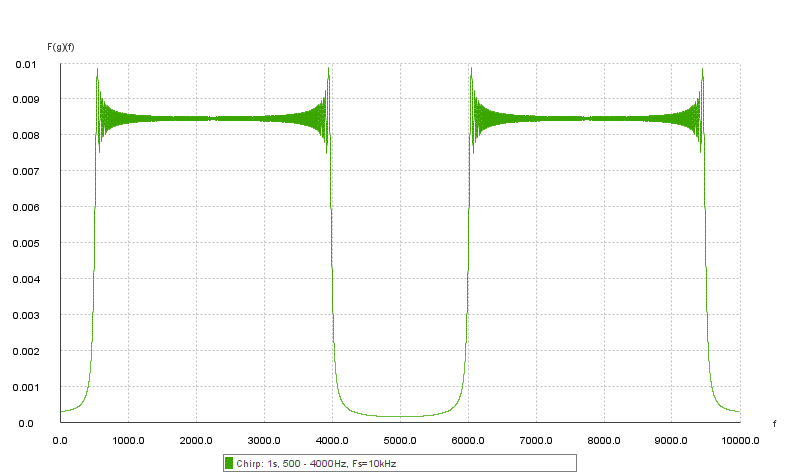
\includegraphics[width=\textwidth]{material/Aufgabe 6.1.3.png}
    \caption{Betragsspektrum $F(g) = |\mathscr{F}(g)|$ des Signals $g$.}
    \end{figure}
    \end{column}
  \end{columns}
\end{frame}
